\documentclass[a4paper, 12pt]{article}
\usepackage[T2A]{fontenc}
\usepackage[utf8]{inputenc}
\usepackage[english,russian]{babel}
\usepackage{amsmath, amsfonts, amssymb, amsthm, mathtools, misccorr, indentfirst, multirow}
\usepackage{wrapfig}
\usepackage{graphicx}
\usepackage{subfig}
\usepackage{adjustbox}
\usepackage{color, colortbl}

\usepackage{geometry}
\geometry{top=20mm}
\geometry{bottom=20mm}
\geometry{left=20mm}
\geometry{right=20mm}

\title{Лабораторная работа 4.2.1\\Кольца Ньютона}
\author{Нехаев Александр\\654 группа}
\date{\today}

\begin{document}
	\maketitle
	\pagenumbering{gobble}
	\newpage
	\tableofcontents
	\pagenumbering{arabic}
	\newpage
	\section{Введение}
	\paragraph{Цель работы:} ознакомление с явлением интерференции в тонких пленках (полосы равной толщины) на примере колец Ньютона и с методикой интерференционных измерений кривизны стеклянной поверхности.
	\paragraph{В работе используются:} измерительный микроскоп с опак-иллюми-натором; плосковыпуклая линза; пластинка из черного стекла; ртутная лампа ПРК-4; щель; линзы; призма прямого зрения; объектная шкала.\par
	В нашей установке кольца Ньютона образуются при интерференции световых волн, отраженных от границ тонкой воздушной прослойки, заключенной между выпуклой поверхностью линзы и плоской стеклянной пластинкой (рис. \ref{calc_scheme}). Наблюдение ведется в отраженном свете.\par
	\begin{wrapfigure}{1}{5cm}
		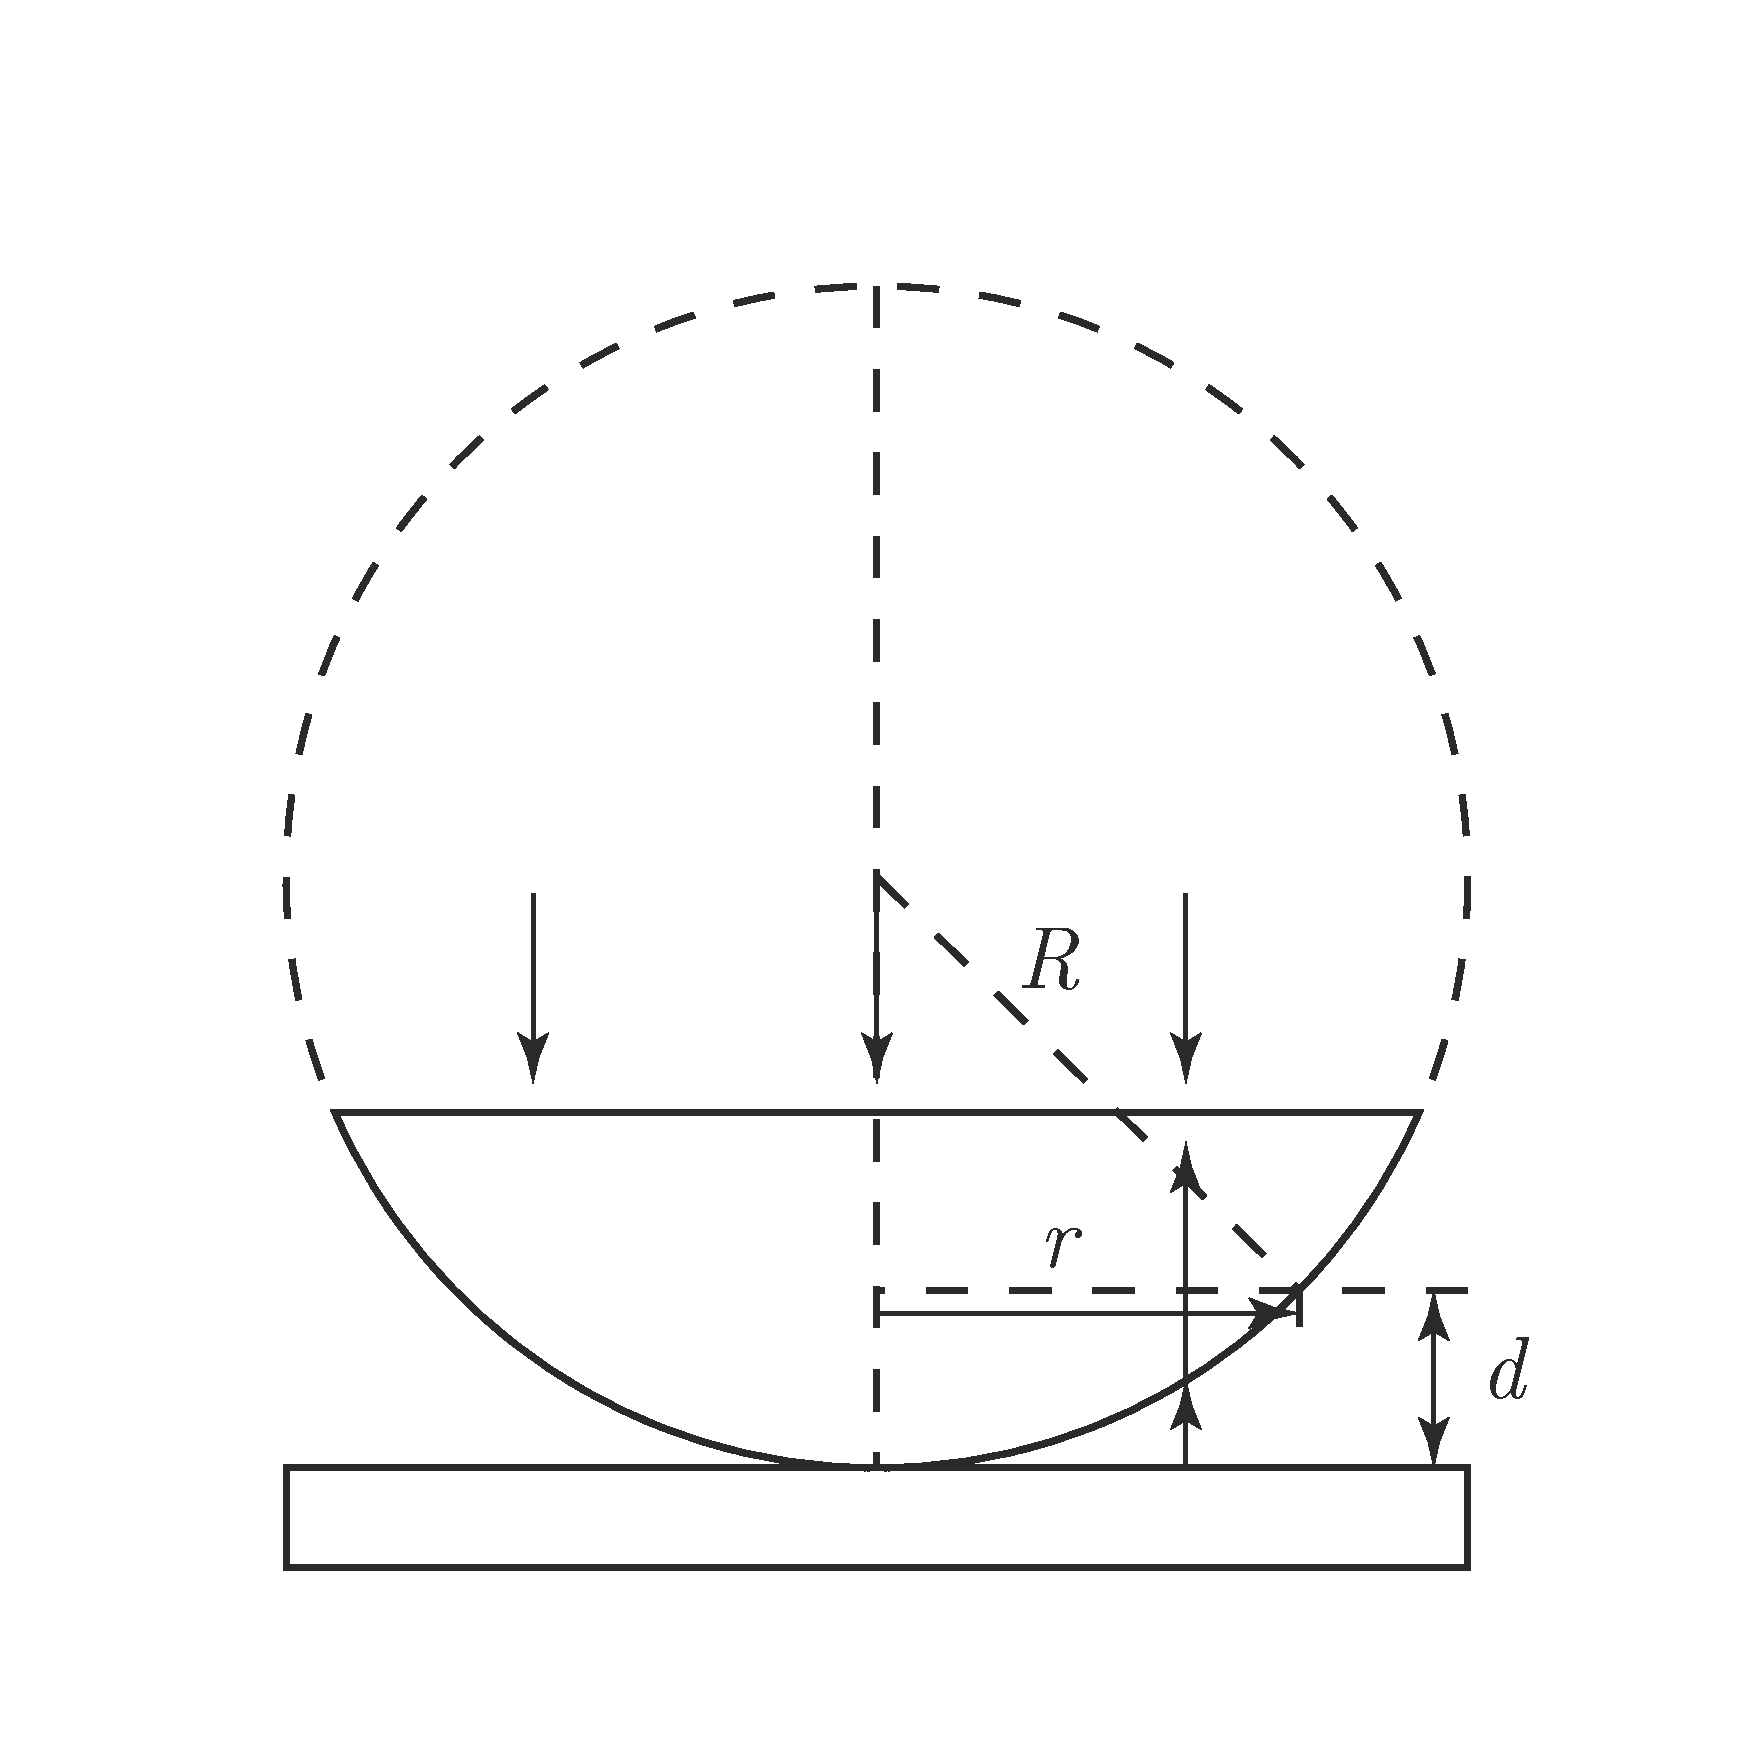
\includegraphics[scale=0.2]{Newton_Rings.pdf}
		\caption{К расчёту колец Ньютона}
		\label{calc_scheme}
	\end{wrapfigure}

	Рассчитаем размер колец Ньютона. Пусть сверху на линзу падает монохроматический параллельный пучок лучей. При вычислении разности хода можно пренебречь небольшими наклонами лучей, проходящих в тонком воздушном зазоре. Геометрическая разность хода между интерферирующими лучами равна, очевидно, $2d$, где $d$ — толщина воздушного зазора в данном месте.\par
	Выразим зависимость $d$ от расстояния $r$ до радиуса, проходящего через точку соприкосновения линзы и пластинки. Из рис. \ref{calc_scheme}. имеем
	\begin{equation*}
		r^2=R^2-\left(R-d\right)^2=2Rd-d^2,
	\end{equation*}
	где R — радиус кривизны выпуклой поверхности линзы. Принимая во внимание, что $2R\gg d$, получим
	\begin{equation}
		d=\frac{r^2}{2R}.
	\end{equation}
	\par
	При вычислении полной разности хода нужно учесть изменение фазы световой волны при отражении от границы стекло-воздух и воздух-стекло. Как известно, для светового (электрического) вектора отражение от оптически более плотной среды происходит с изменением фазы на $\pi$. Свет, отраженный от границы стекло—воздух, по сравнению со светом, отраженным от границы воздух—стекло, приобретает, таким образом, дополнительный фазовый сдвиг на $\pi$, что соответствует разности хода $\lambda/2$. Полная разность хода $\Delta$ равна
	\begin{equation}
		\Delta=2d+\frac{\lambda}{2}=\frac{r^2}{R}+\frac{\lambda}{2}.
		\label{way_delta_eq}
	\end{equation}
	Линии постоянной разности хода представляют собой концентрические кольца с центром в точке соприкосновения. При заданном значении длины волны $\lambda$ разность хода $\Delta$ определяется толщиной воздушного зазора; интерференционные полосы являются, таким образом, линиями равной толщины.\par
	Известно, что линии равной толщины для точечного источника света не имеют области локализации: их можно наблюдать в любом месте пространства, где пересекаются лучи, отражённые от двух поверхностей. Для протяжённого источника линии равной толщины локализованы на поверхности клина (в нашем случае на поверхности воздушной прослойки). Это означает, что при освещении системы не вполне параллельным пучком света (что практически всегда имеет место) интерференционные полосы оказываются наиболее четкими при фокусировке на верхнюю поверхность воздушного клина.\par
	Запишем условие минимума освещенности в интерференционной картине:
	\begin{equation}
		\Delta=\left(2m+1\right)\frac{\lambda}{2}, \quad m=0,1,2, ...
	\end{equation}
	Принимая во внимание (\ref{way_delta_eq}), получим для радиусов $r_m$ темных колец
	\begin{equation}
		r_m=\sqrt{mR\lambda}.
		\label{dark_ring_radius_eq}
	\end{equation}
	Аналогичным образом для радиусов $r_m'$ светлых колец найдем
	\begin{equation}
		r_m'=\sqrt{\left(2m-1\right)R\lambda/2}.
		\label{light_ring_radius_eq}
	\end{equation}
	\par
	Измеряя радиусы светлых или темных колец, с помощью (\ref{dark_ring_radius_eq}) и (\ref{light_ring_radius_eq}) можно определить $\lambda$, если известен радиус $R$ кривизны линзы, или, наоборот, по известному значению $\lambda$ найти $R$.
	\section{Экспериментальная установка}
	\begin{wrapfigure}{1}{5cm}
		\centering
		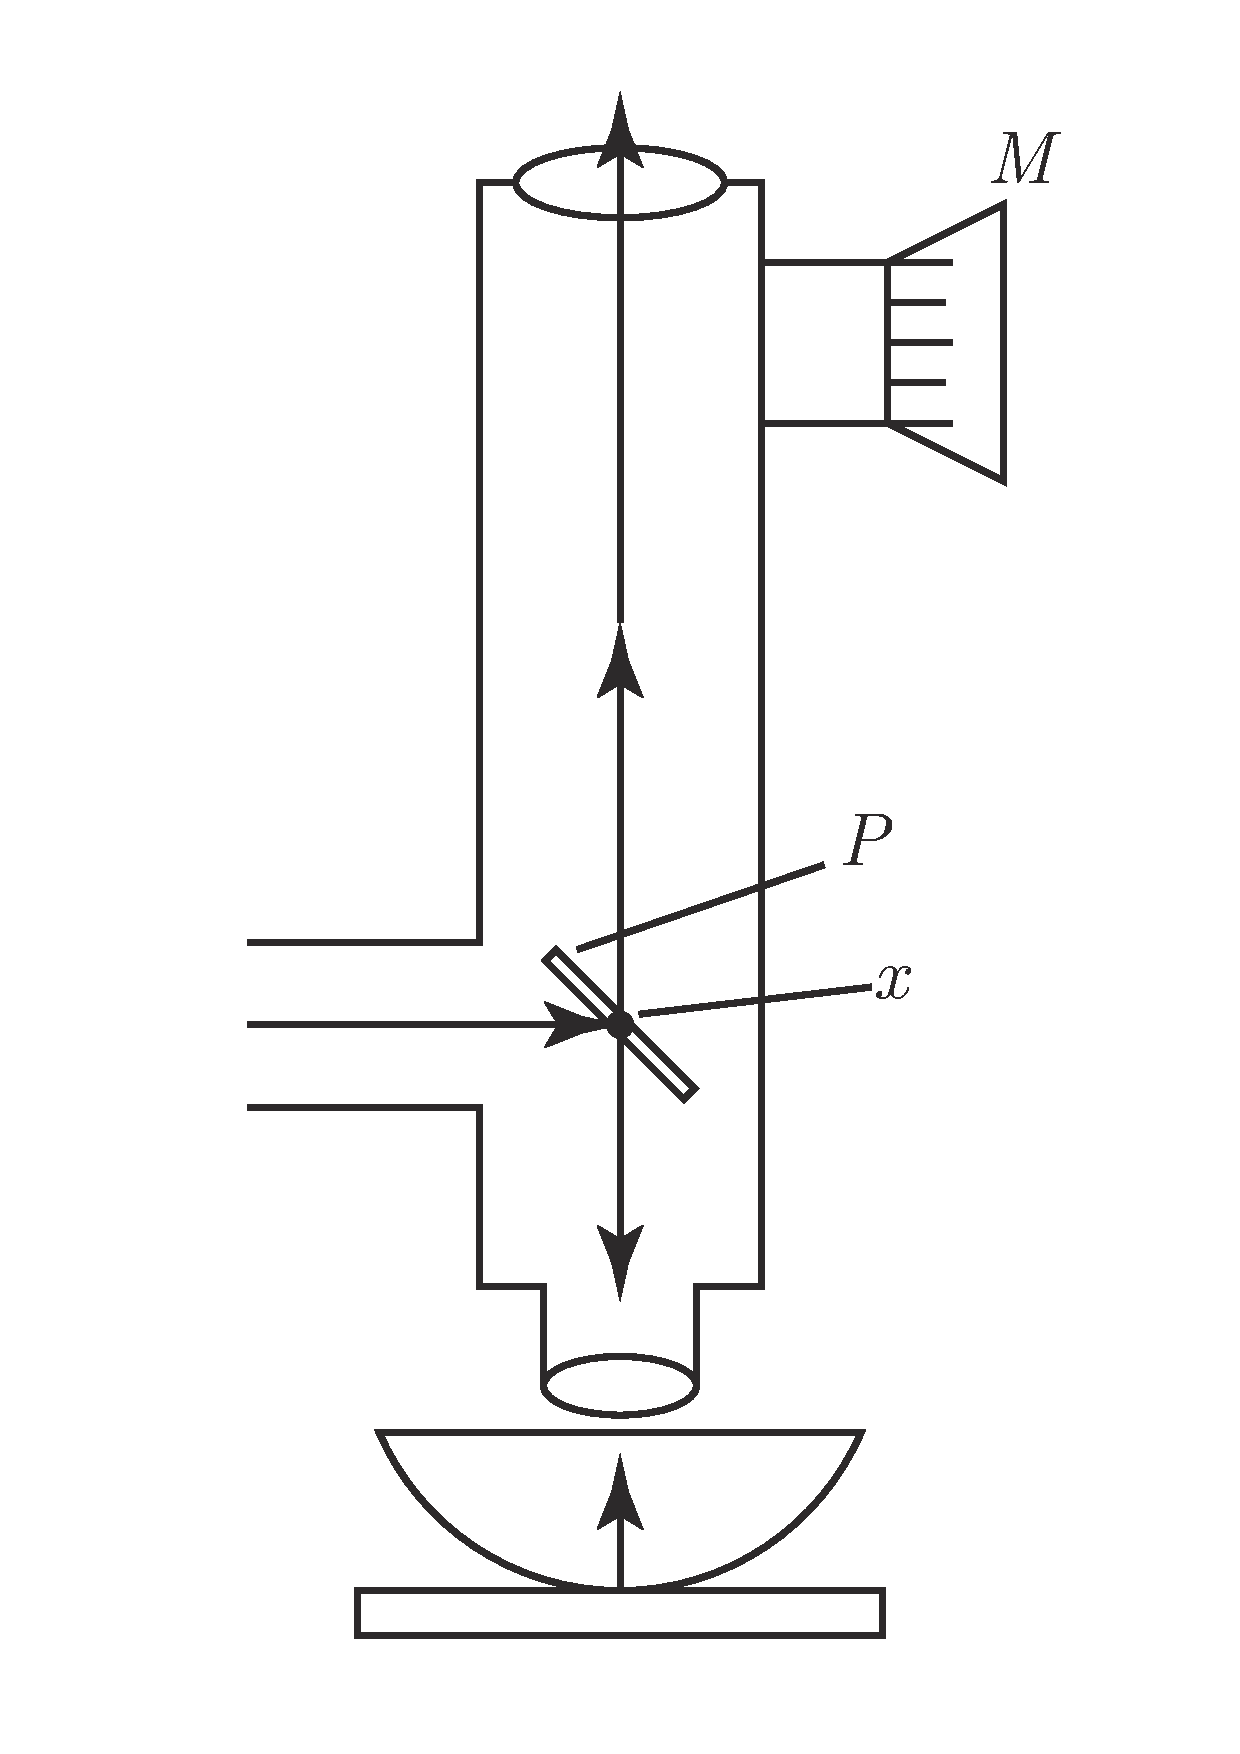
\includegraphics[scale=0.19]{Microscope.pdf}
		\caption{Освещение линзы с помощью опак-иллюминатора}
		\label{lense_illumination}
	\end{wrapfigure}
	Опыт выполнятся с помощью измерительного микроскопа помещается держатель с полированной пластинкой из черного стекла (рис. \ref{lense_illumination}). На пластинке лежит исследуемая линзы.\par
	Между окуляром и объективом микроскопа расположен опак-иллюминатор — специальное устройство, служащее для освещения объекта при работе в отраженном свете. Внутри опак-иллюминатора находится полупрозрачная стеклянная пластинка $P$, наклоненная под углом $45^\circ$ к оптической оси микроскопа. Свет от расположенного сбоку источника частично отражается от этой пластинки, проходит через объектив микроскопа и попадает на исследуемый объект. Пластинка может поворачиваться вокруг горизонтальной оси $x$.\par
	Столик микроскопа может перемещаться в двух взаимно перпендикулярных направлениях при помощи специальных винтов — препаратоводителей,\par
	При измерениях окуляр перемещается перпендикулярно оптической оси с помощью микрометрического винта $M$.\par
	Источником света служит ртутная лампа (типа ПРК-4), находящаяся в защитном кожухе. Для монохроматизации света (для выделения одной или нескольких спектральных линий, используемых для освещения) применяется призменный монохроматор (рис. \ref{monochrom_scheme}), состоящий из конденсатора $K$, щели $S$, объектива $O$ и призмы прямого зрения $\Pi$. Все эти устройства с помощью рейтеров располагаются на оптической скамье.\par
	\begin{wrapfigure}{1}{6cm}
		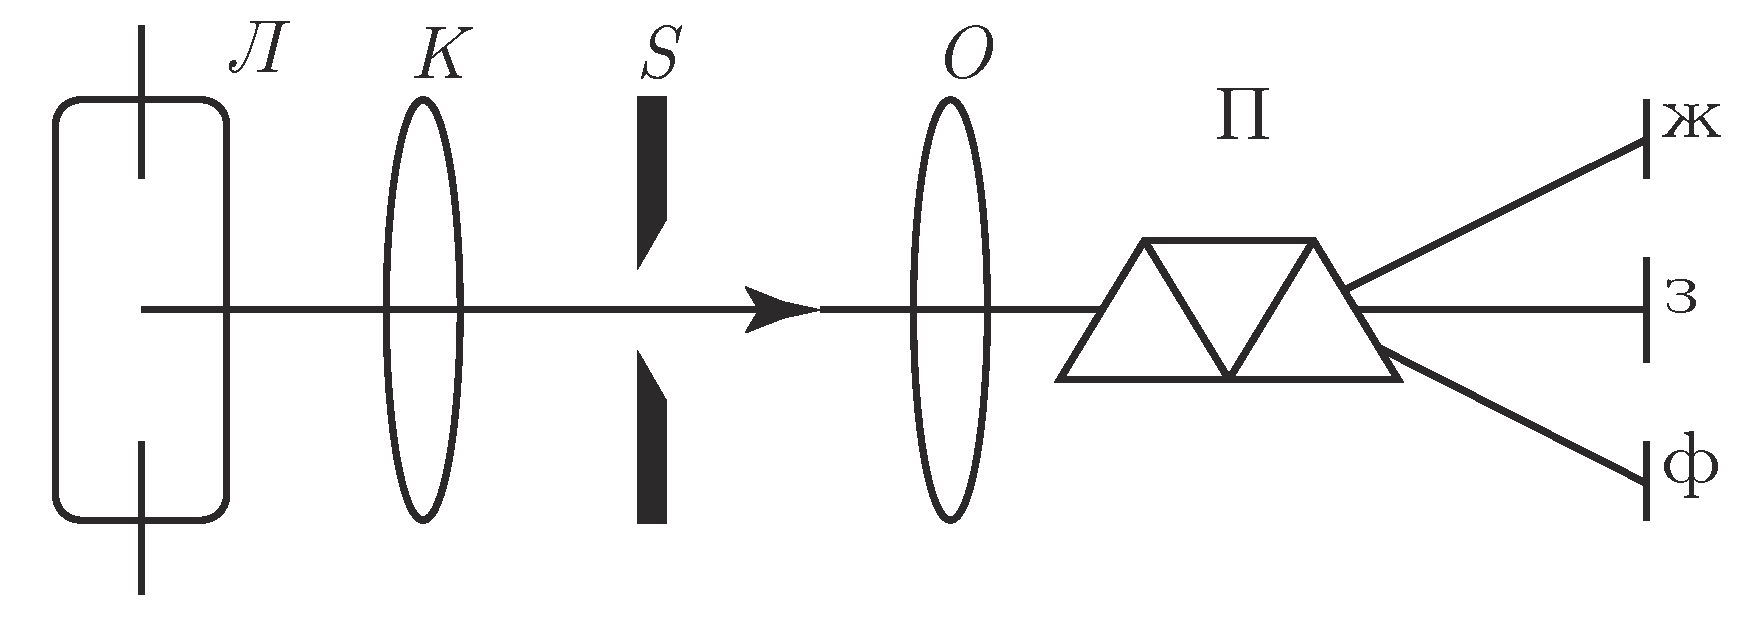
\includegraphics[scale=0.2]{Scheme.pdf}
		\caption{Схема устройства монохроматора}
		\label{monochrom_scheme}
	\end{wrapfigure}

	Оптическая система позволяет получить в плоскости входного окна опак-иллюминатора достаточно хорошо разделённые линии спектра ртутной лампы.\par
	Рекомендуется сначала настроить микроскоп на кольца Ньютона в белом свете (свете ртутной лампы), затем пи помощи монохроматора выделить из ртутного спектра яркую зелёную линию и провести измерения диаметров колец в монохроматическом свете.
	\section{Ход работы}
	\begin{enumerate}
		\item Включим ртутную лампу и настроим микроскоп на кольца Ньютона в белом свете.
		\item Настроим монохроматор, фокусируя на входного окне опак-иллюминатора изображение зеленой линии ртути.
		\item Вращая окулярный микрометрический винт, убедимся, что перекрестие проходит через центр тёмного пятна и что поле зрения освещено симметрично слева и справа от центра.\par
			Определим координаты диаметров тёмных и светлых колец. Результаты измерений занесем в таблицу \ref{diameters_table} (темные пятна соответствуют темному фону):
			\definecolor{Gray}{gray}{0.9}
			\begin{table}[h]
				\centering
				\begin{tabular}{|c|c|}
					\hline
					Слева от пятна & Справа от пятна\\
					\hline
					\rowcolor{Gray}
					0.23 & 5.38\\
					0.31 & 5.32\\
					\rowcolor{Gray}
					0.40 & 5.23\\
					0.48 & 5.14\\
					\rowcolor{Gray}
					0.56 & 5.04\\
					0.67 & 4.99\\
					\rowcolor{Gray}
					0.75 & 4.85\\
					0.86 & 4.76\\
					\rowcolor{Gray}
					0.96 & 4.62\\
					1.05 & 4.49\\
					\rowcolor{Gray}
					1.18 & 4.40\\
					1.32 & 4.26\\
					\rowcolor{Gray}
					1.48 & 4.10\\
					1.64 & 3.92\\
					\rowcolor{Gray}
					1.84 & 3.76\\
					2.15 & 3.50\\
					\hline
				\end{tabular}
				\caption{Координаты диаметров темных и светлых колец.}
				\label{diameters_table}
			\end{table}
		\item Оценим диаметр пятна соприкосновения линзы со стеклянной пластинкой.
		\begin{equation*}
			d=3.27-2.39=0.88 \text{ дел}.
		\end{equation*}
%		\begin{figure}[h]
%			\centering
%			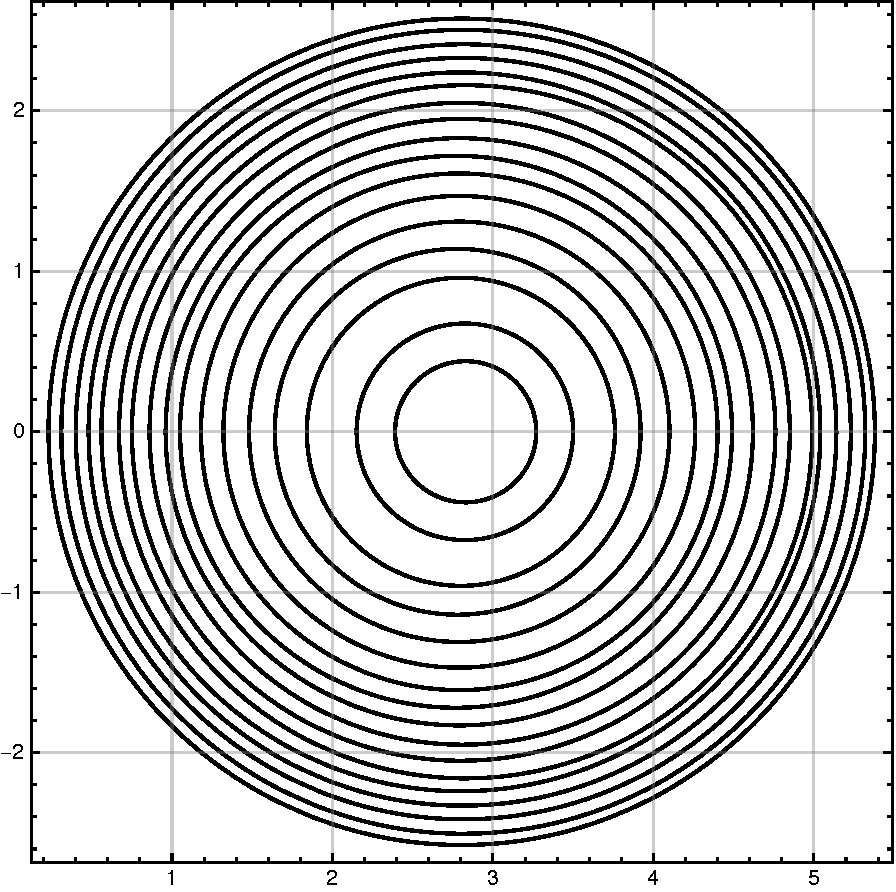
\includegraphics[scale=0.5]{Newton_Rings_Restored_Scientific.pdf}
%			\caption{Восстановленная картина колец Ньютона.}
%		\end{figure}
		\item Проведем наблюдение биений для жёлтой и зелёной линий, оценим разность длин волн и сопоставим результат с табличным.\par
			Зарегистрировали $m=16$ колец для зеленой спектральной линии. Тогда
			\begin{equation*}
				m=\frac{\lambda}{\Delta\lambda},\quad \Delta\lambda=\frac{\lambda}{m}=\frac{546}{16}=34.125 \text{ нм}.
			\end{equation*}
			Спектральные линии ртути желтого и зеленого цветов соответственно имеют длины волн $\lambda_\text{жел}=579\text{ нм}$, $\lambda_\text{зел}=546\text{ нм}$. Тогда $\Delta\lambda=33$ нм, что близко к полученному значению.
		\item Прокалибруем окулярную шкалу, используя эталонную объективную шкалу. Объектная шкала размером 1 мм разбита на 100 делений. Между делениями "2" и "3" окулярной шкалы $9\pm0.5$ делений объектной шкалы. Значит цена одного деления окулярной шкалы равно $\frac{(1\pm0.5)\text{ мм}}{100}\cdot 9=(9.0\pm0.05)\cdot10^{-2}$ мм.
		\item Рассчитаем радиусы тёмных и светлых колец и построим графики зависимости $r_m^2$ и $(r_m')^2$ от номера кольца $m$.\par
			Координата центра пятна: $\frac{3.27-2.39}{2} + 2.39=(2.830\pm0.005)$ дел.
			Формула для расчета $r_{m}^2$ имеет вид:
			\begin{equation*}
				r_{m}^2=\frac{\left((x_1-x_c)\cdot a\right)^2+\left((x_2-x_c)\cdot a\right)^2}{2},
			\end{equation*}
			где $x_1$ — левая координата кольца, $x_2$ — правая координата кольца, $x_c$ — координата центра пятна, $a$ — цена деления объективной шкалы.
			\begin{table}[h]
				\centering
				\begin{tabular}{|c|c|c|c|c|}
					\hline
					$m$ & $r_{m}^2$ $\cdot 10^{-2}$ мм$^2$ & $\sigma r_{m}^2$ $\cdot 10^{-2}$ мм$^2$ & $(r_{m}')^2$ $\cdot 10^{-2}$ мм$^2$ & $\sigma (r_{m}')^2$ $\cdot 10^{-2}$ мм$^2$\\
					\hline
					1 & 0.747 & 0.023 & 0.369 & 0.005 \\
 					2 & 1.391 & 0.042 & 1.054 & 0.046 \\
 					3 & 2.100 & 0.052 & 1.751 & 0.047 \\
 					4 & 2.713 & 0.059 & 2.399 & 0.083 \\
 					5 & 3.404 & 0.050 & 3.080 & 0.031 \\
 					6 & 4.064 & 0.054 & 3.779 & 0.005 \\
 					7 & 4.724 & 0.029 & 4.397 & 0.038 \\
 					8 & 5.371 & 0.052 & 5.082 & 0.030 \\
 					\hline
				\end{tabular}
				\caption{Квадраты радиусов темных и светлых колец.}
			\end{table}
			\begin{figure}[h]
				\centering
				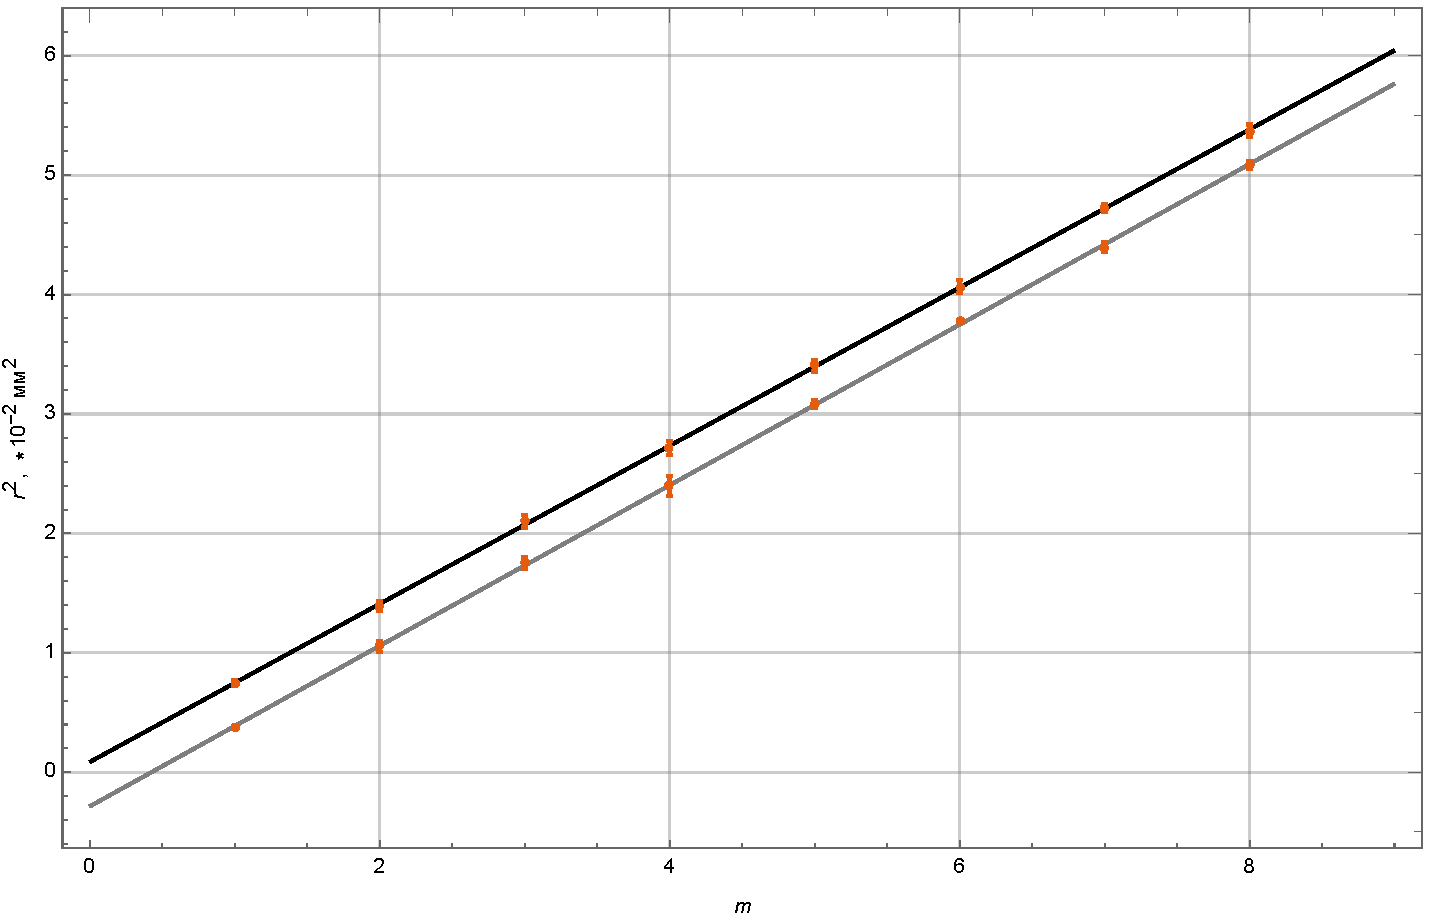
\includegraphics[scale=0.7]{Graphic.pdf}
				\caption{График зависимости $r^2$ от номера кольца для темных и светлых колец.}
			\end{figure}
			\par
			По графику определим наклон прямых:
			\begin{equation*}
				y=0.662 x+0.085,\quad y=0.672 x-0.286
			\end{equation*}
			Для линии темных колец: $\tan\alpha_{1}=0.662\pm 0.003$, для светлых: $\tan\alpha_{2}=0.672\pm 0.003$.\par
			Из формул (\ref{dark_ring_radius_eq}) и (\ref{light_ring_radius_eq}) находим, что радиус линзы через темные кольца:
			\begin{equation*}
				R_\text{ч}=\frac{r_m^2}{m\lambda}=\frac{\tan\alpha_1}{\lambda}=\frac{0.662\cdot10^{-2} \text{ мм}^2}{546\text{ нм}}=(12.13\pm0.05) \text{ мм}.
			\end{equation*}
			\begin{equation*}
				R_\text{с}=\frac{(r_m')^2}{(2m-1)\lambda}=\frac{\tan\alpha_2}{\lambda}=\frac{0.672\cdot10^{-2} \text{ мм}^2}{546\text{ нм}}=(12.31\pm0.05)\text{ мм}.
			\end{equation*}
			Усредняя полученные значения получим
			\begin{equation*}
				R=(12.216\pm0.104)\text{ мм}.
			\end{equation*}
			График для темных колец проходит через начало координат, следовательно размытия нет.
			\section{Вывод}
			Ознакомились с явлением интерференции в тонких пленках на примере колец Ньютона и с методикой интерференционных измерений кривизны стеклянной поверхности. Смогли рассчитать радиус кривизны линзы $R=(12.216\pm0.104)\text{ мм}.$
	\end{enumerate}
\end{document}
